%%% Local Variables:
%%% mode: latex
%%% TeX-master: "../doc"
%%% coding: utf-8
%%% End:
% !TEX TS-program = pdflatexmk
% !TEX encoding = UTF-8 Unicode
% !TEX root = ../doc.tex
\section{Aufgabenstellung}
\label{sec:aufgabenstellung}
\begin{figure}[H]
  \centering
  
\includegraphics[page=1,scale=0.55]{../ressources/Aufgabenstellung.pdf}
\end{figure}
\begin{figure}[H]
  \centering

\includegraphics[page=2,scale=0.55]{../ressources/Aufgabenstellung.pdf}
\end{figure}


\section{Packages}
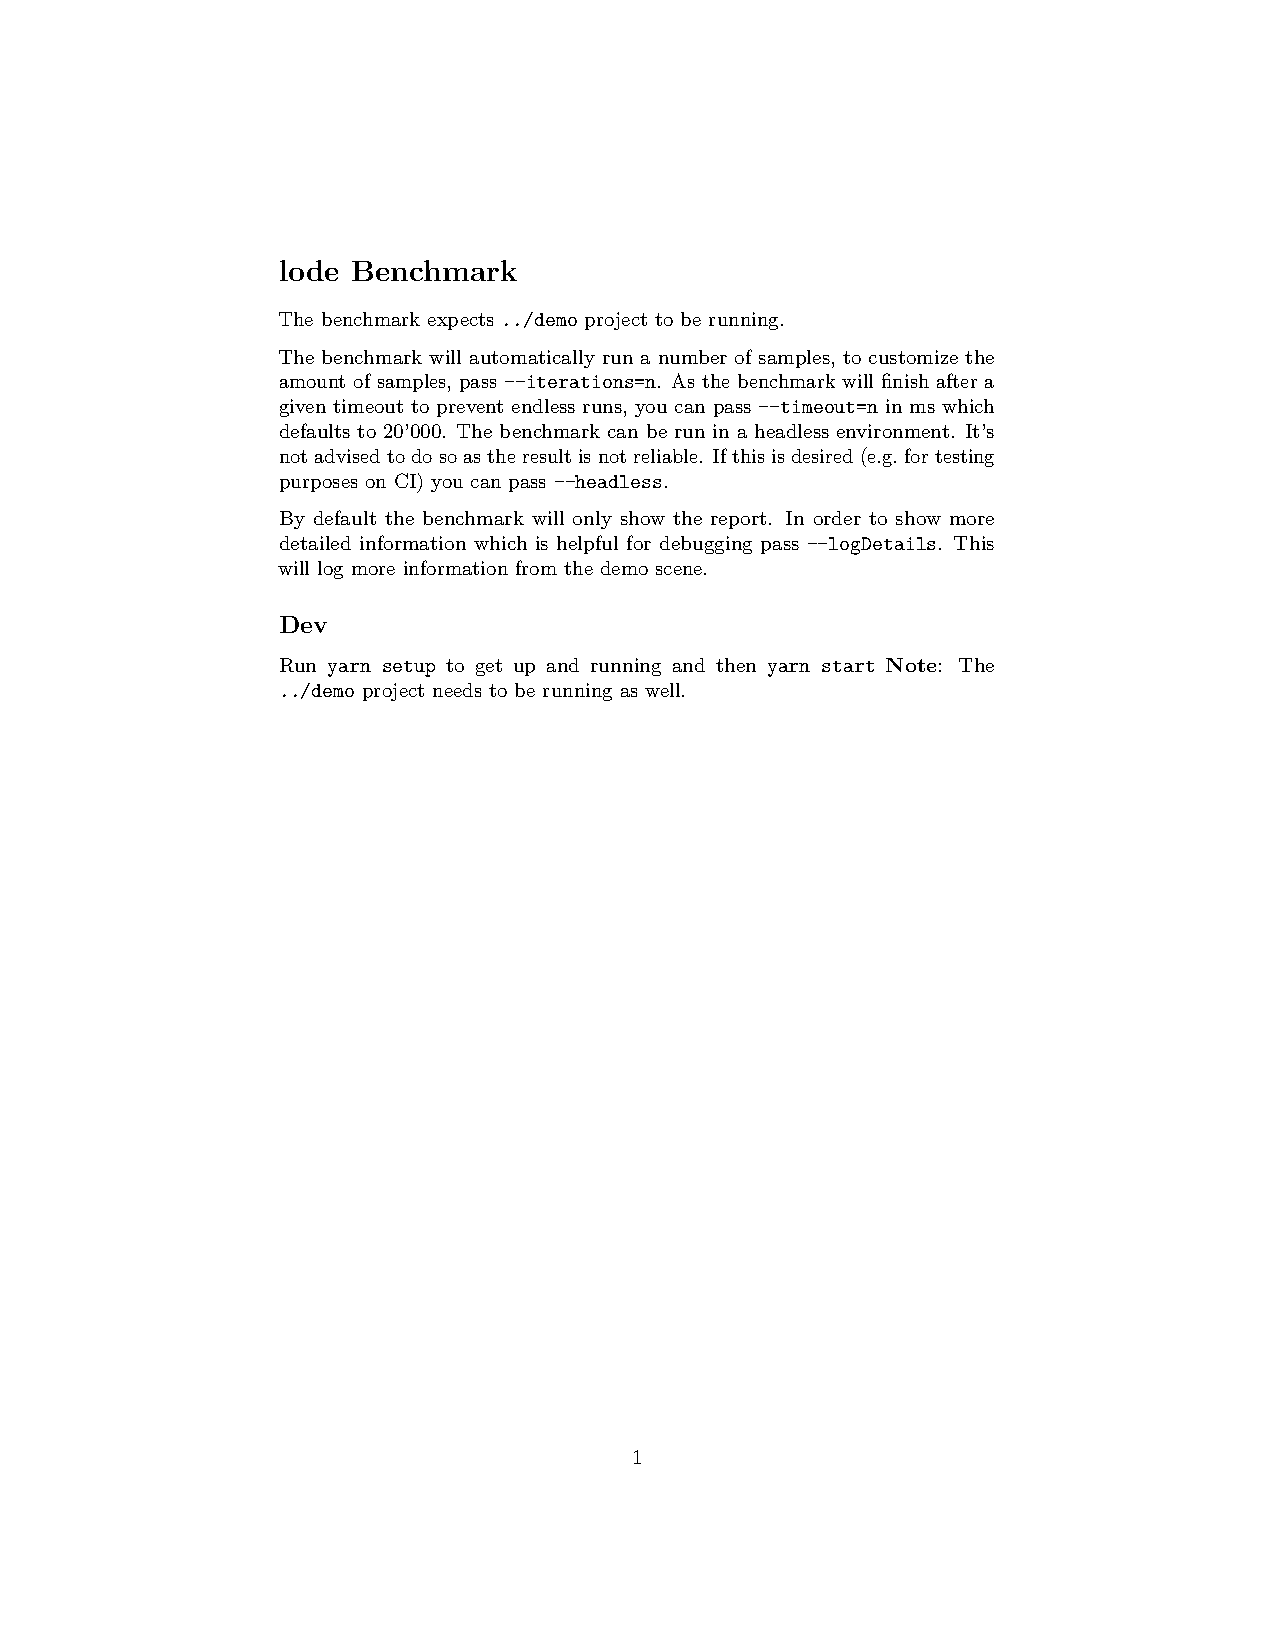
\includepdf[pagecommand={},scale=0.92,pages=-]{../ressources/packages/benchmark.pdf}
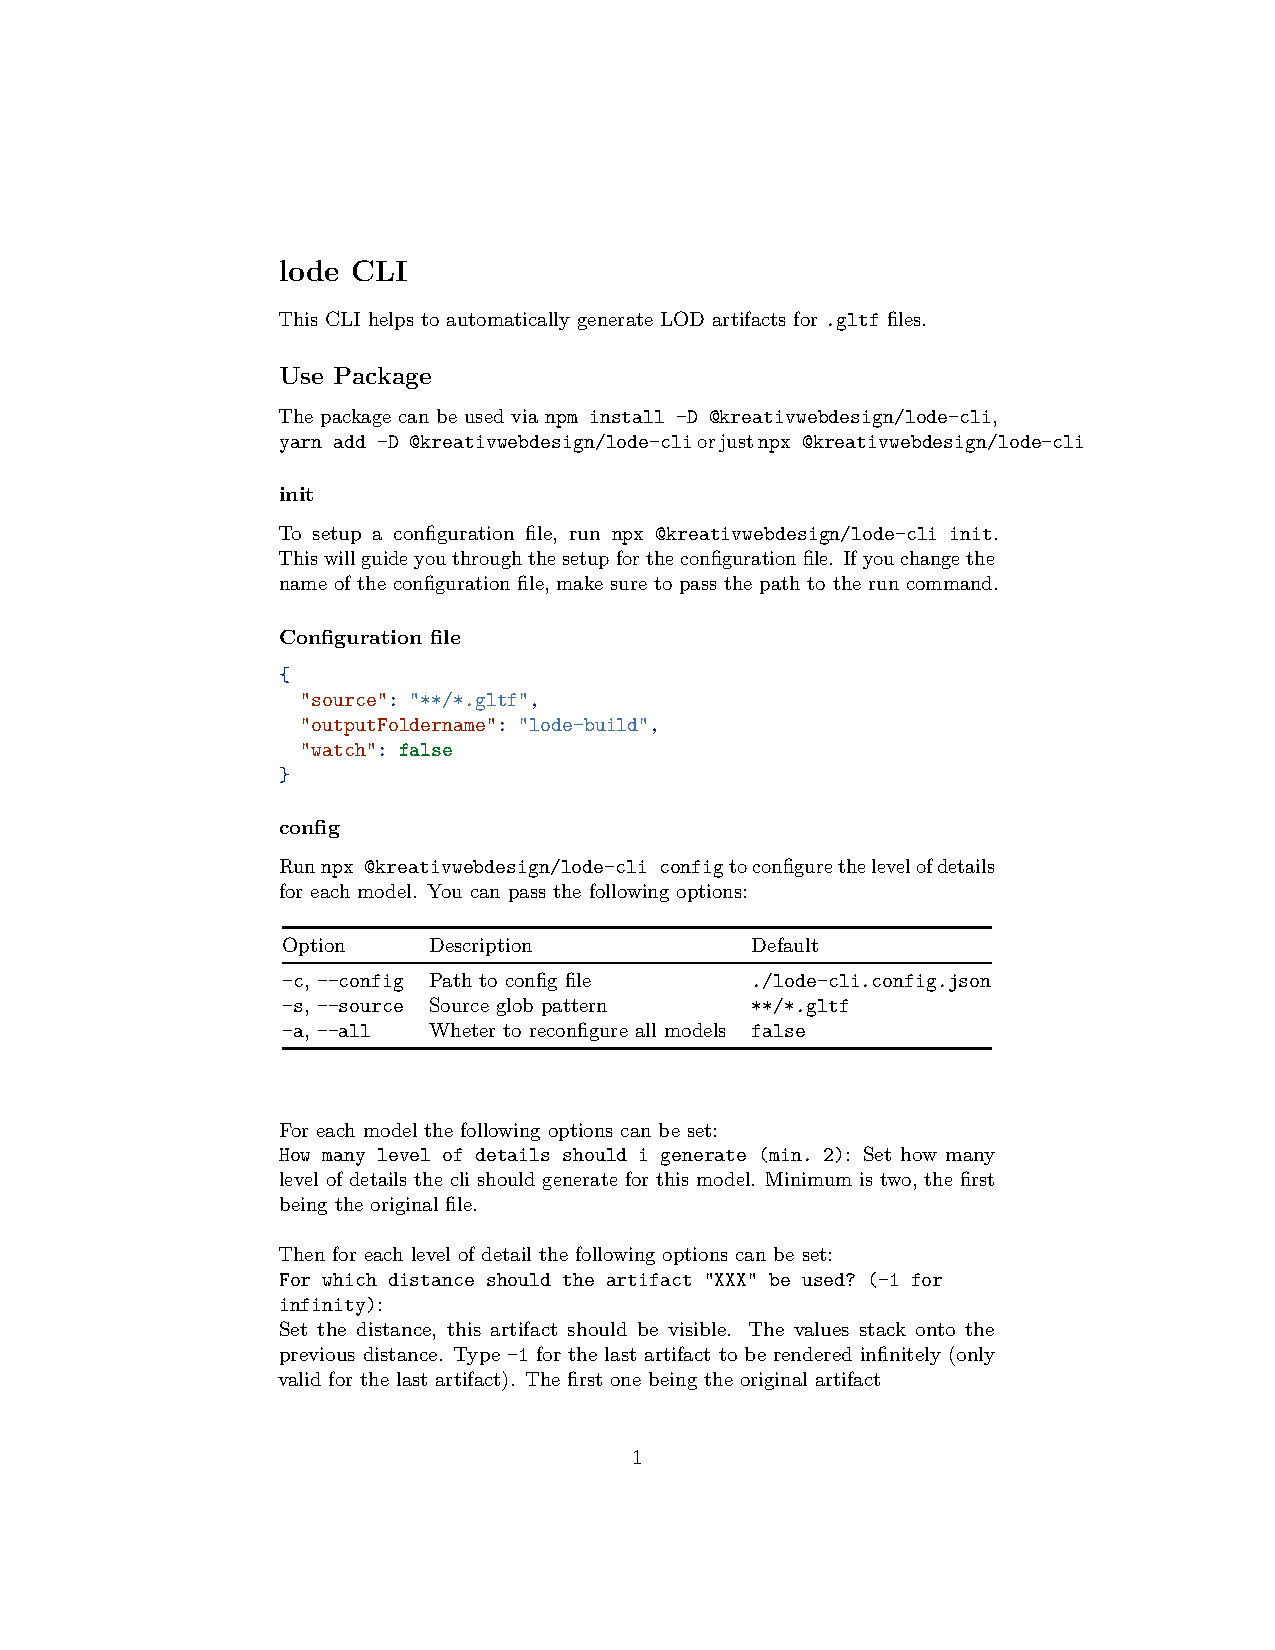
\includepdf[pagecommand={},scale=0.92,pages=-]{../ressources/packages/cli.pdf}
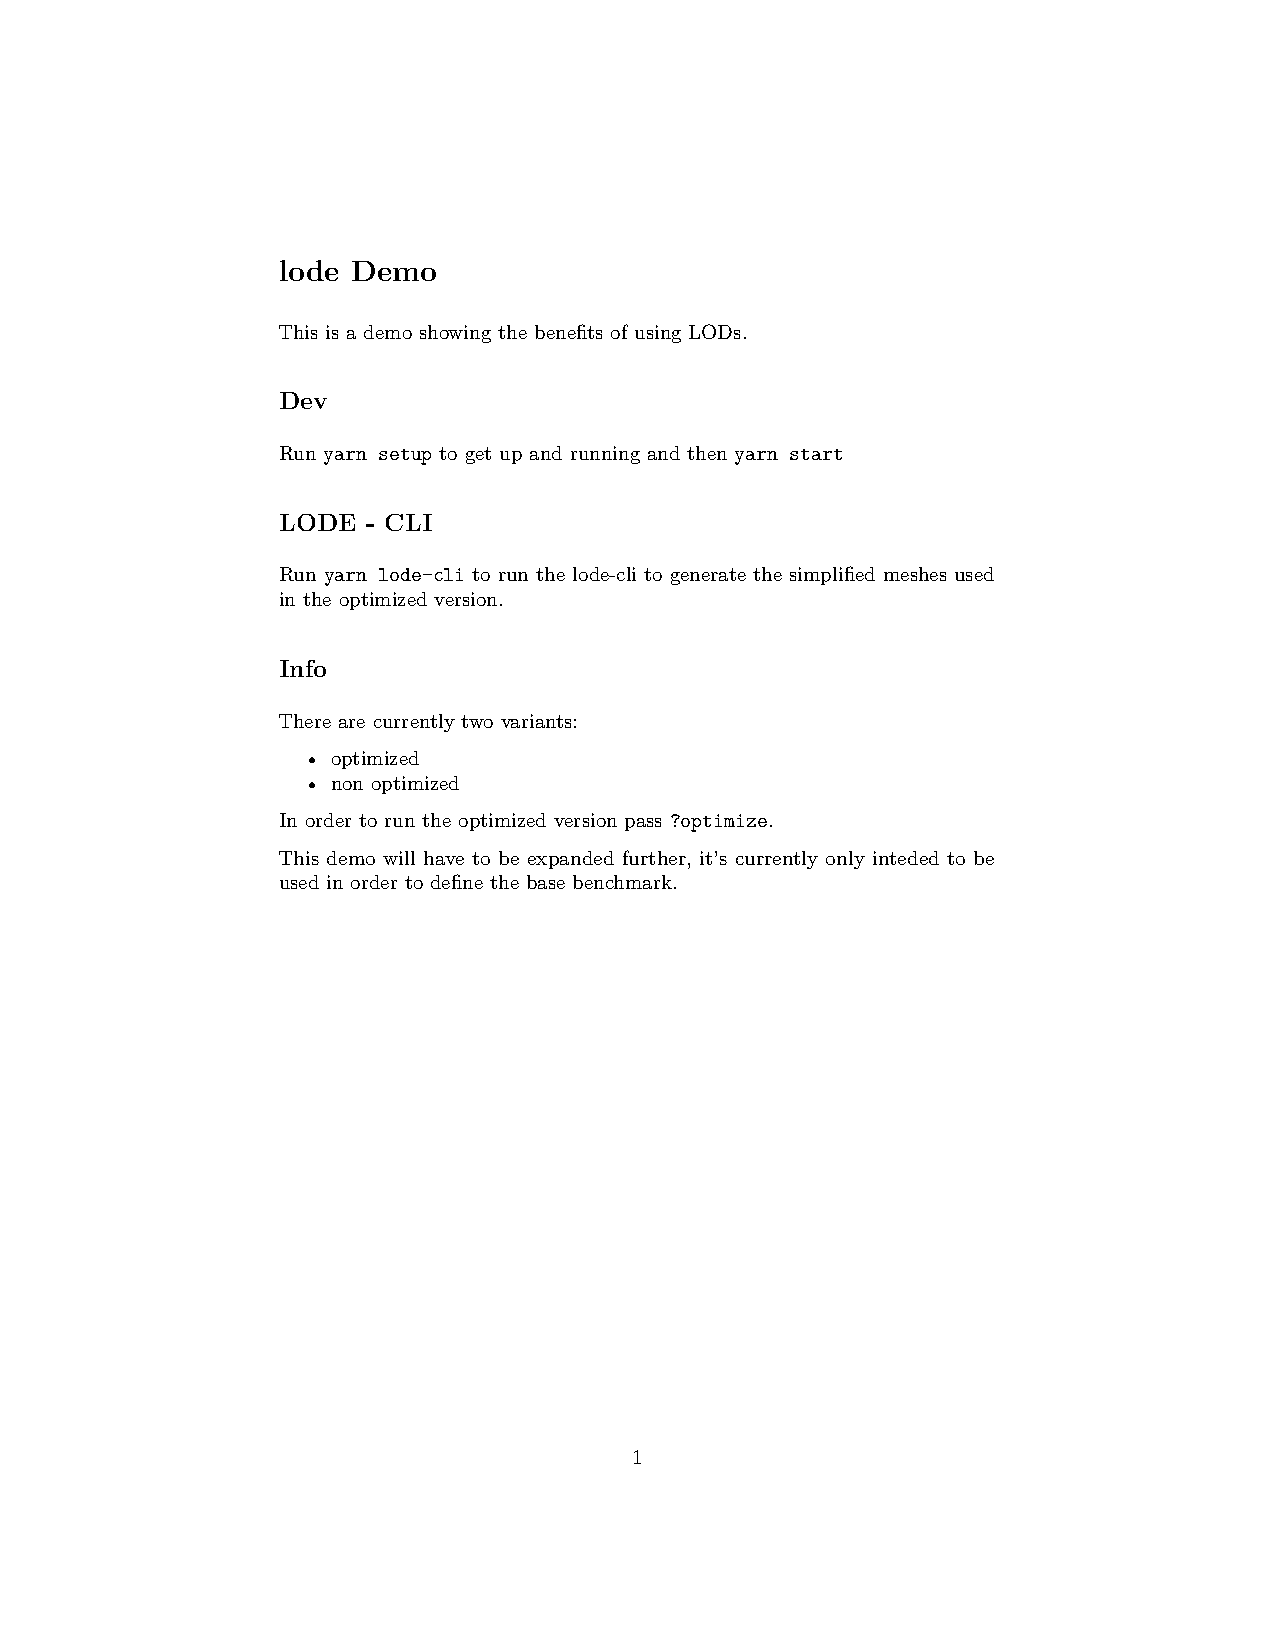
\includepdf[pagecommand={},scale=0.92,pages=-]{../ressources/packages/demo.pdf}
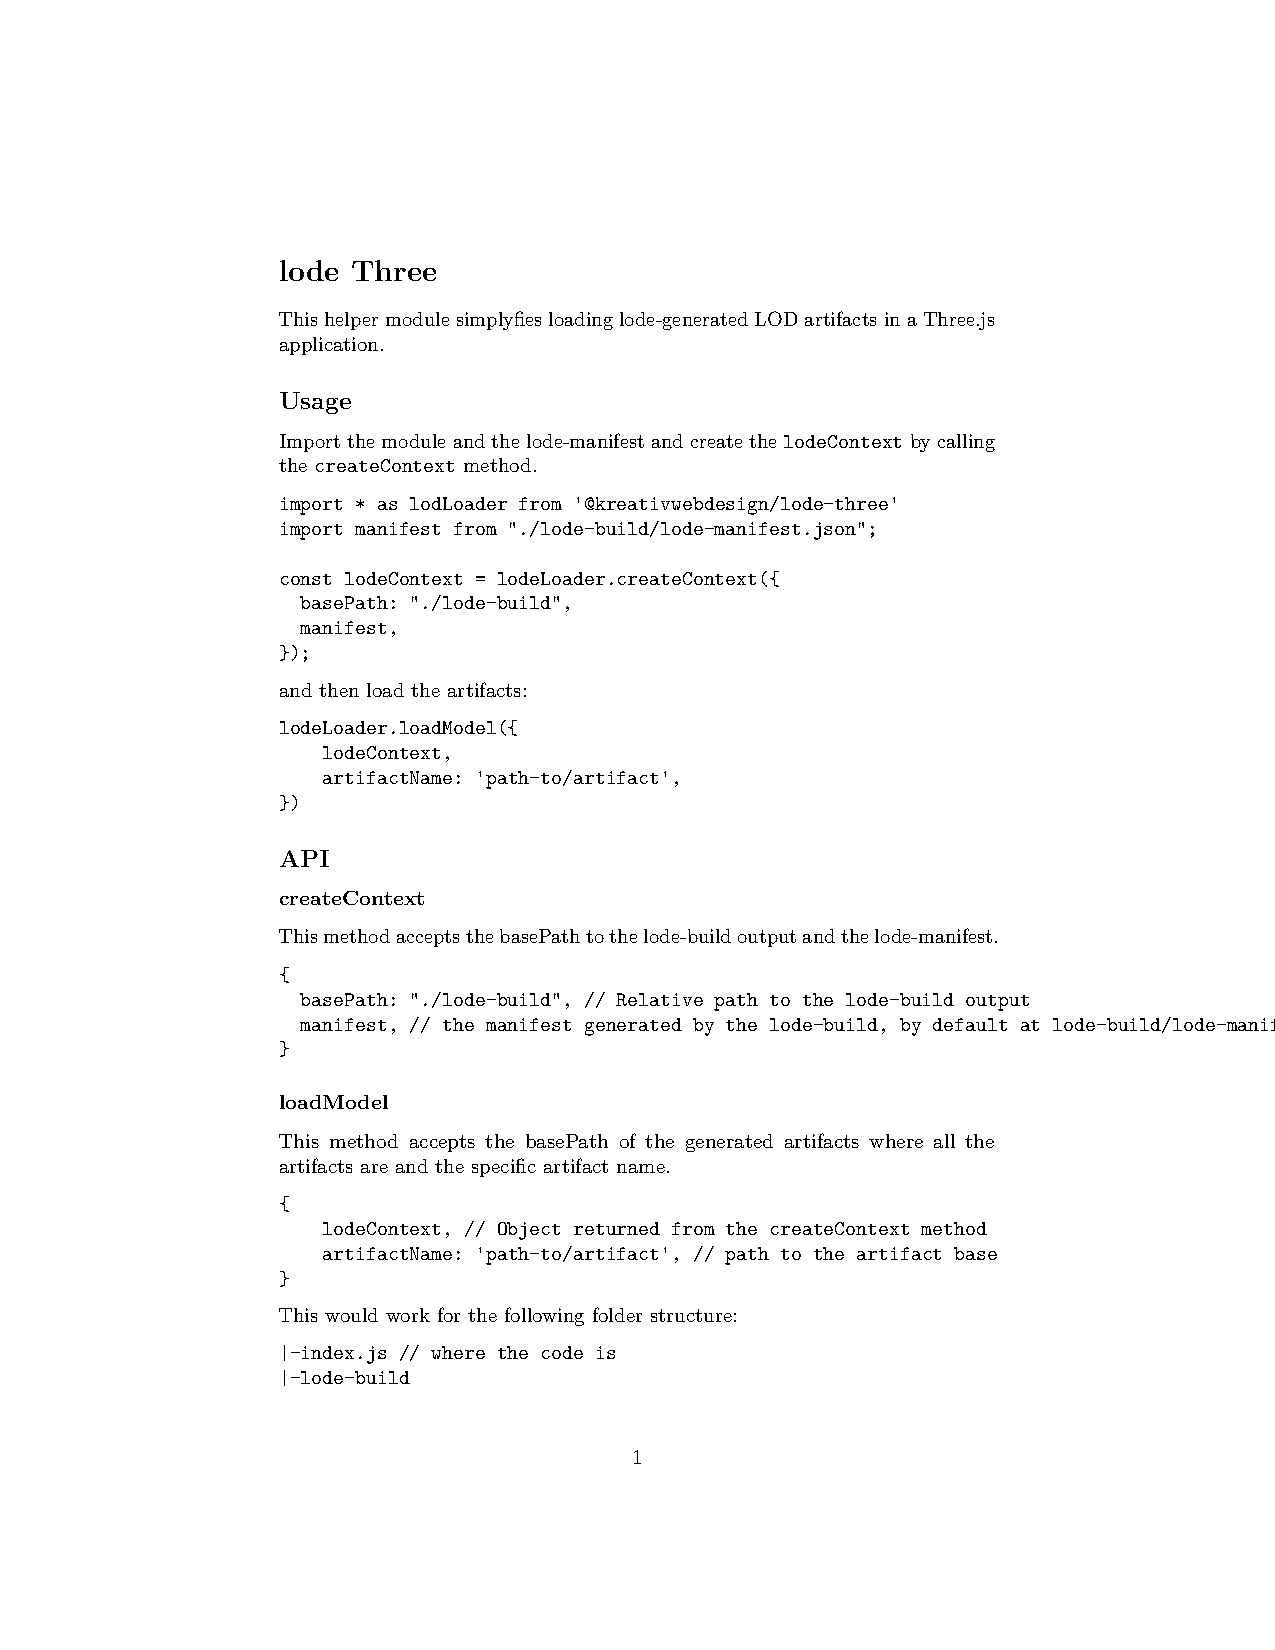
\includepdf[pagecommand={},scale=0.92,pages=-]{../ressources/packages/lode-three.pdf}
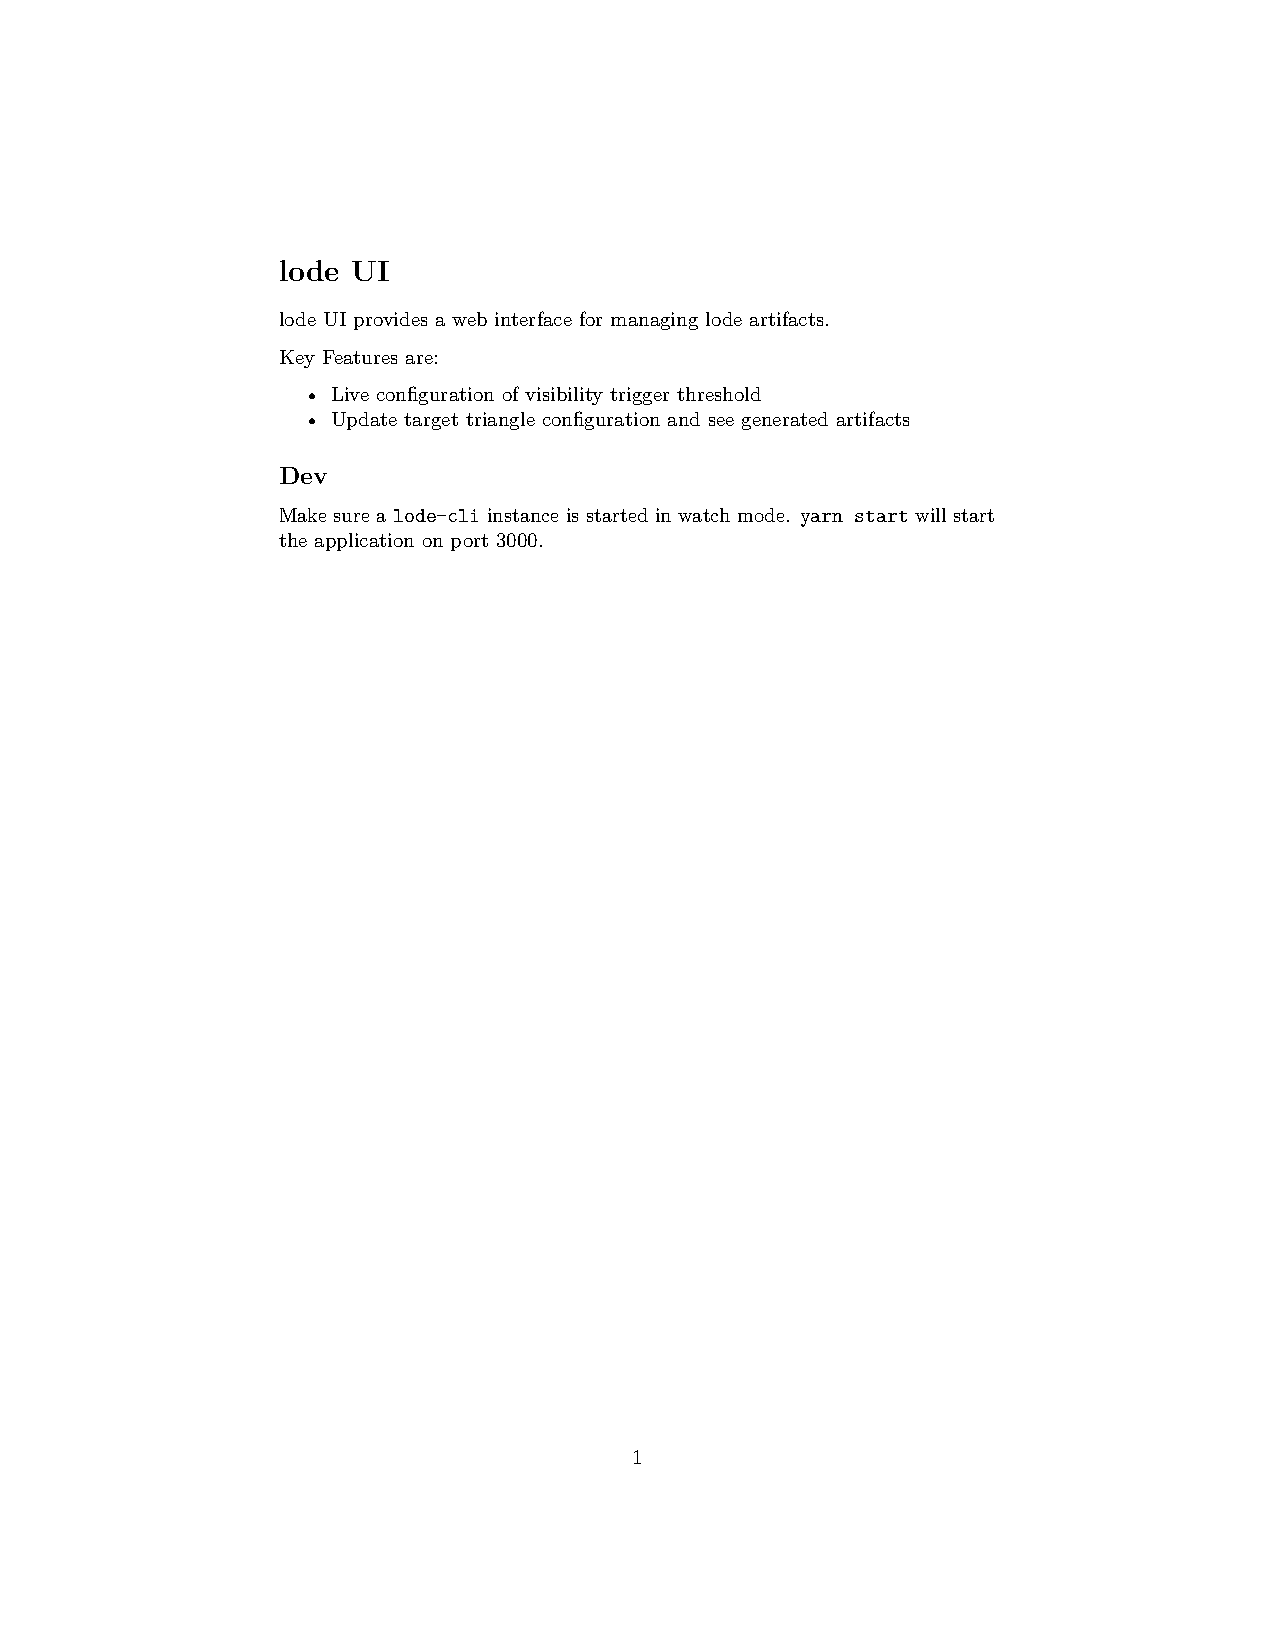
\includepdf[pagecommand={},scale=0.92,pages=-]{../ressources/packages/lode-ui.pdf}
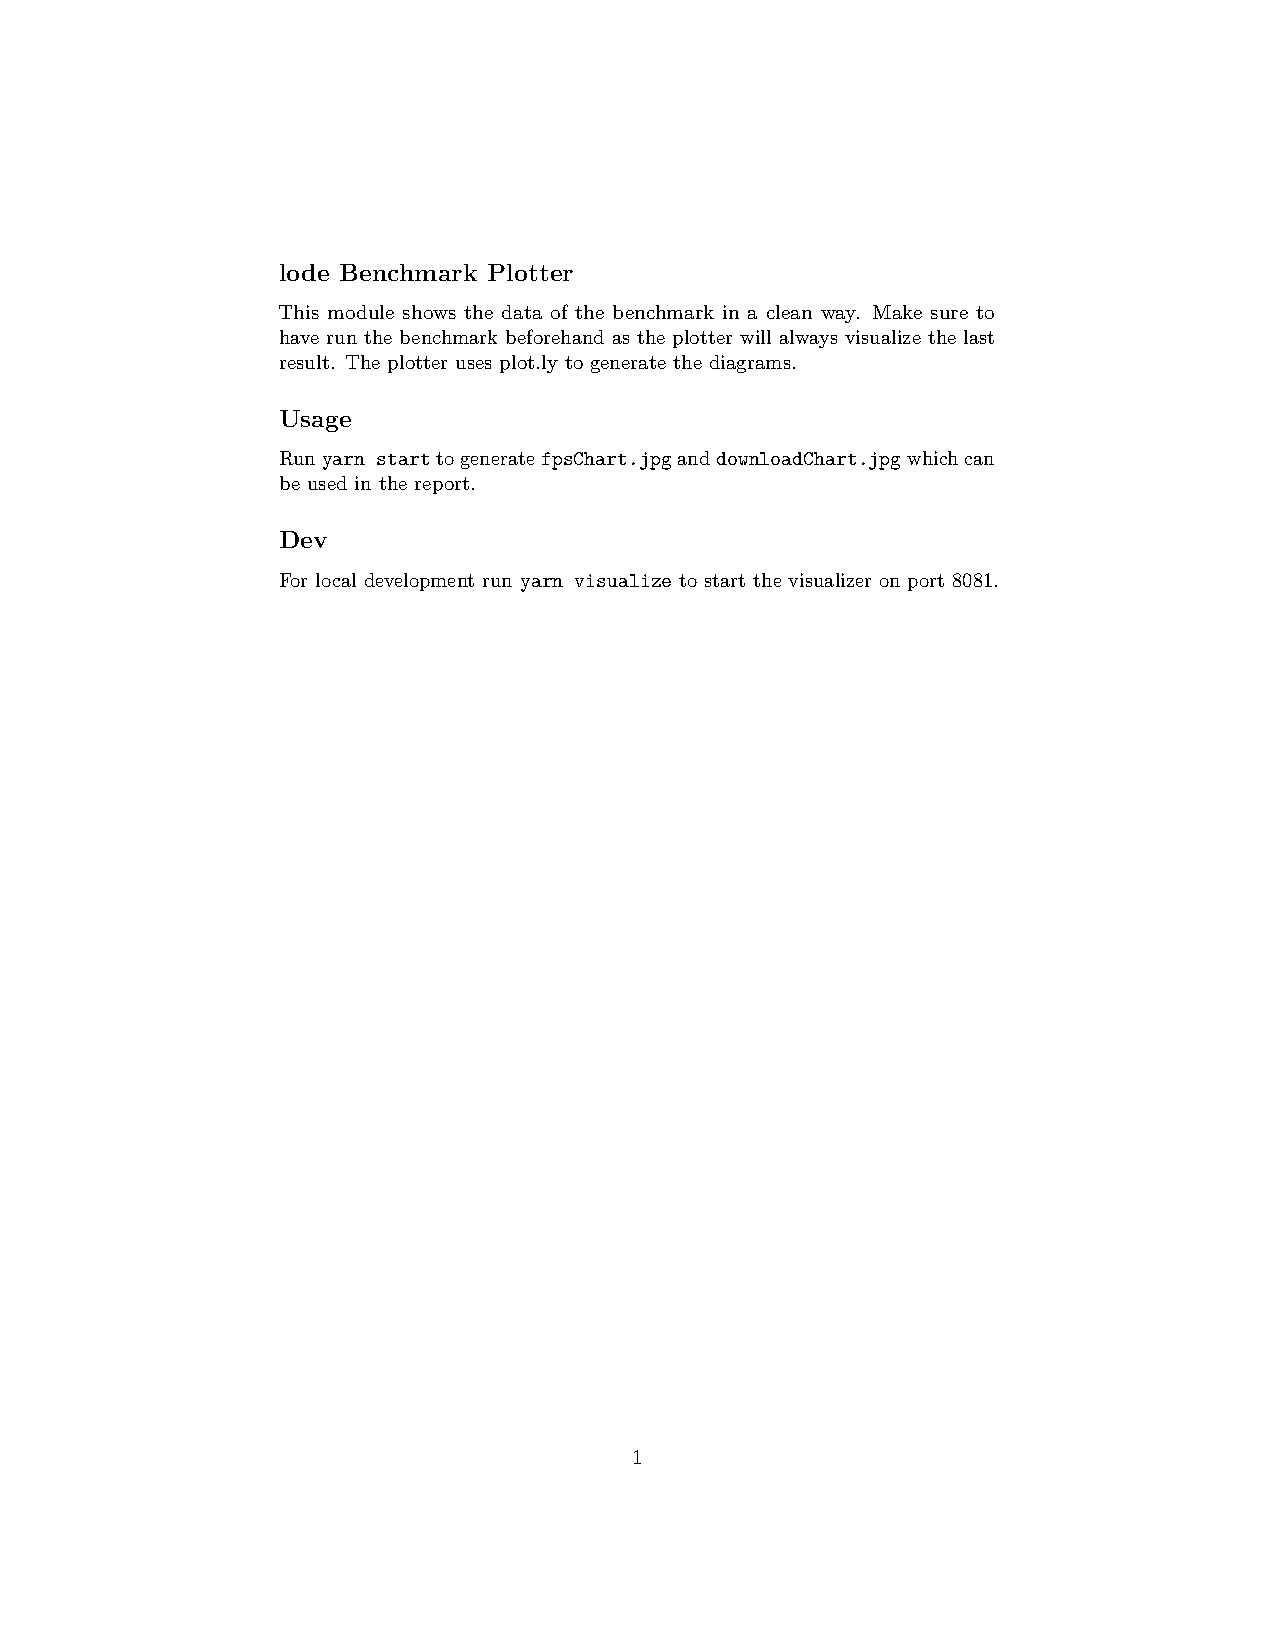
\includepdf[pagecommand={},scale=0.92,pages=-]{../ressources/packages/plotter.pdf}
